\chapter{Digital Elastica minimization via graph cuts}
\label{chapter:graphflow}

In the previous chapter we have defined the concept of balance coefficient that motivate us to introduce the BalanceFlow model. In fact, the balance coefficient is also present in the FlipFlow energy and it seems that its computation is in the core of the evolution processes described so far. We confirm this hypothesis once more in this chapter. We present a graph-based model that converges to the optimum digital shape in the free digital Elastica problem. Moreover, the model is easily adapted for image segmentation tasks.

\section{Standard graph-cut segmentation}
The Grabcut model \cite{rother04grabcut} partitions an image in foreground and background components by computing minimum cuts in a graph. The model is very attractive, as minimum cuts are fastly computed for sparse graphs. We start by giving some necessary definitions from graph theory.

\subsection{Definitions}

\begin{definition}{Unordered graph}
The unordered graph $\mathcal{G}(\mathcal{V},\mathcal{E})$ is a pair of sets $\mathcal{V},\mathcal{E}$ such that $\mathcal{V}$ is finite and $\mathcal{E}$ is a collection of unordered pairs of $\mathcal{V}$, i.e., 

\begin{align*}
\mathcal{E} \subseteq  \left\{ \; \{x,y\} \; | \; x,y \in \mathcal{V} \; \right\}.
\end{align*}

\end{definition}

\begin{definition}{Connected graph}
The graph $\mathcal{G}(\mathcal{V},\mathcal{E})$ is connected if for every pair of vertices $v,u$ there exists a path $\pi$ of length $n$ such that

\begin{align*}
	v_1 = v, \quad v_n = u, \quad 	\pi = \left\{ v_i \; | \; \{v_{i-1},v_{i}\} \subset \mathcal{E} \right\},\quad  2<i<n.
\end{align*}
\end{definition}

A digital set $S \subset \Omega \subset \mathbb{Z}^2$ is naturally represented as a graph $\mathcal{G}(\mathcal{V},\mathcal{E})$ by letting each pixel $p \in S$ to correspond to a vertex $v_p \in \mathcal{V}$. The set of edges is defined accordingly with the application in mind. Moreover, one can define a cost function $w:\mathcal{E}\rightarrow \mathbb{R}$ on the edge set. In this case, we speak of a weighted graph.

\begin{definition}{Cut}
Let $\mathcal{G}(\mathcal{V},\mathcal{E})$ a connected graph weighted  by cost function $w:\mathcal{E}\rightarrow \mathbb{R}$. A cut set is a subset $\mathcal{E}' \subset \mathcal{E}$ such that the graph $\mathcal{G}(\mathcal{V},\mathcal{E} \setminus \mathcal{E}')$ is disconnected. Moreover, the cut value of $\mathcal{E}'$ is defined as

\begin{align*}
	cut(\mathcal{E}) &= \sum_{e \in \mathcal{E}'}{w(e)}.
\end{align*}
\end{definition}

We are interested on $(s,t)$-cuts, i.e., cuts in which vertices $s,t$ are disconnected after the cut set is removed. We denote $s,t$ as the source and target vertices, respectively. 

%Cuts are a natural way to partition a digital shape in two disjoint sets. In the GrabCut algorithm, the images are partitioned in foreground and background. In the context of shape evolution, we partition the vertices in: those belong to $S$ (connected to source) and those who do not belong to $S$ (connected to target).

The Grabcut model consists in a judicious definition of the cost function $w$ in order to segment objects in a digital image accordingly with its color intensity values.

\subsection{Grabcut binary segmentation model}
Let $I:\Omega\rightarrow [0,1]^3$ to represent a $3$-channel colored image. Consider the graph $\mathcal{G}(\mathcal{V},\mathcal{E})$ defined as

\begin{align*}
	\mathcal{V} &= \left\{ v_p \; | \; \forall p \in \Omega \right\} \cup \{s,t\}\\
	\mathcal{E} &= \mathcal{E}_{st} \cup \mathcal{E}_{\mathcal{N}},
\end{align*}
where 
\begin{align*}
\mathcal{E}_{st} &= \left\{ \{s,v_p\}, \{t,v_p\} \; | \; \forall p \in \mathcal{V}  \right\} \\
\mathcal{E}_{\mathcal{N}} &= \left\{ \{v_p,v_q\} \; | \; \forall p\big( p \in \mathcal{V} \text{ and } q\in \mathcal{N}_4(p) \big)  \right\}.
\end{align*}

Next, let sets $\mathcal{V_F}, \mathcal{V_B} \subset \mathcal{V}$ to represent foreground and background seeds input by the user. Vertices in $\mathcal{V_F}$ ($\mathcal{V_B}$) are forced to be connected to the source (target) after the removal of the minimum cut set.

Consider the functions
\begin{align*}
	B(\{v_p,v_q\}) &= exp \left( -\frac{ (I(p) - I(q))^2}{2\sigma ^2} \right) \\
	R(v_p,``bg") &= -ln H_B(p)\\
	R(v_p,``fg") &= -ln H_F(p),
\end{align*}

where $H_B,H_F$ are mixed Gaussian distributions derived from  foreground and background seeds given by the user; and $\sigma$ is interpreted as a parameter to configure noise level of the input image.

Finnaly, define the cost function $w:\mathcal{E}\rightarrow \mathbb{R}$ as

\begin{table}[H]
\centering
\setlength{\extrarowheight}{0.75em}
\begin{tabular}{|c|c|c|}
\hline
\textbf{edge} $e$ & $\mathbf{w(e)}$ & \textbf{for}\\
\hline
$\{v_p, v_q\}$ & $B(e)$ & $e \in \mathcal{E}_{\mathcal{N}}$\\
\hline
\multirow{3}{*}{$\{v_p, s\}$} & $\lambda_r R(v_p,\text{``bg"})$ & $p \in \mathcal{\mathcal{V}}, p \notin \mathcal{\mathcal{V}}_F \cup \mathcal{\mathcal{V}}_B$\\
& M & $p \in \mathcal{\mathcal{V}}_F$ \\
& 0 & $p \in \mathcal{\mathcal{V}}_B$ \\
\hline
\multirow{3}{*}{$\{v_p, t\}$} & $\lambda_r R(v_p,\text{``fg"})$ & $p \in \mathcal{\mathcal{V}}, p \notin \mathcal{\mathcal{V}}_F \cup \mathcal{\mathcal{V}}_B$\\
& 0 & $p \in \mathcal{\mathcal{V}}_F$ \\
& M & $p \in \mathcal{\mathcal{V}}_B$ \\
\hline
\end{tabular}
\begin{align*}
\text{where,} \qquad M = 1 + \max_{p \in \Omega}{\sum_{q \in \mathcal{N}_4(p)}}{B(\{p,q\})}.
\end{align*}
\end{table}

Let $\mathcal{E}'$ the minimum cut of $\mathcal{G}$ and $C$ the connected component of $\mathcal{G}$ induced by $\mathcal{E}'$ that contains the source vertex. The grabcut energy value is given by

\begin{align*}
	grab_{\Lambda}(C) &= \lambda_r \cdot \Big( \sum_{p \in C}{R(v_p,"fg")} + \sum_{p \in \overline{X}}{R(v_p,"bg")} \Big) + \lambda_b \cdot \sum_{e \in \mathcal{E}'}{B(e)}.
\end{align*}


The Grabcut segmentation is heavily impacted by the quality of the input image. To attenuate the problem, one could extend the Grabcut model by defining a cost function that takes geometric information into account. Indeed, the work \cite{boykov03geodesics} describes a cost function in which one could do image segmentation with length regularization. There exist some attempts \cite{nieuwenhuis14efficient,zehiry10fast} to inject curvature information in a graph-cut framework, but the models present issues on running time and lack precision on the estimation of curvature. In the next section we describe a graph-cut model that uses the balance coeficient to regularize curvature.


\section{GraphFlow model}
Given some energy $E$, the GraphFlow model is divided in two main steps: candidate selection and validation. At the candidate selection step, a minimum cut is computed for each member of a set of candidate graphs. From the minimum cuts we derive candidate solutions for the minimization of $E$. The validation step consists in select the candidate solution with the lowest value of $E$.

The GraphFlow model is suitable for the free, constrained Elastica problem and image segmentation. In particular, the GraphFlow model is a simple extension of the Grabcut model for image segmentation that regularizes the squared curvature.

In the next sections, we are going to describe the GraphFlow model that aims to minimize the energy

\begin{align}
E^{graph} &= \hat{E}_{\Theta} + grab_{\Lambda}.
\label{eq:graphflow-energy}
\end{align}


\subsection{The candidate graph}

%Let $I:\Omega \rightarrow [0,1]^3$ a $3$-channel colored image and $S$ a digital set representing a initial foreground partition of image $I$. 

Let $S \subset \Omega \subset \mathbb{Z}^2$ a digital set. Given $n>0$, we define the optimization band $O_n(S)$ as

\begin{align*}
	O_n(S) &:=\left\{ p \in \Omega \; | \; -n <= d_{S}(p) \leq n \right\}.
\end{align*}

We are going to construct the candidate graph $\mathcal{G}_n(S) = ( \mathcal{V},\mathcal{E})$. The vertex and edge sets are defined as 

\begin{align*}
	\mathcal{V} &= \{ v_p \; | \; p \in S \cup O_n \} \cup \{s,t\} \\
	\mathcal{E} &= \mathcal{E}_{st} \cup \mathcal{E}_\mathcal{N}.
\end{align*}

where $s,t$ are the source and target vertices, respectively. As in the previous section, sets $\mathcal{V}_F,\mathcal{V}_B \subset \mathcal{V}$ correspond to foreground and background seeds input by the user. Additionaly, we define the sets

\begin{align*}
	\mathcal{V}_s &= \left\{ v_p \; | \; p \in S \setminus O_n(S) \right\}\\
	\mathcal{V}_t &= \left\{ v_p \; | \; p \in \overline{S} \setminus O_n(S) \right\}.
\end{align*}

The sets $\mathcal{V}_s, \mathcal{V}_t$ are going to be forced to be connected to source and target components, respectively. The cost function $w:\mathcal{E}\rightarrow \mathbb{R}$ is defined as 

\begin{table}[H]
\centering
\setlength{\extrarowheight}{0.75em}
\begin{tabular}{|c|c|c|}
\hline
\textbf{edge} $e$ & $\mathbf{w(e)}$ & \textbf{for}\\
\hline
$\{v_p, v_q\}$ & $\beta \big(u(S,p) + u(S,q)\big) + \lambda_bB(e)$ & $p,q \in \mathcal{E}_{\mathcal{N}}$\\
\hline
\multirow{3}{*}{$\{v_p, s\}$} & $\lambda_r R(v_p,\text{``bg"})$ & $p \in \mathcal{\mathcal{V}}, p \notin \mathcal{\mathcal{V}}_F \cup \mathcal{\mathcal{V}}_B \cup \mathcal{\mathcal{V}}_s \cup \mathcal{\mathcal{V}}_t$\\
& $\lambda_r M_1\mathbbm{1}(\mathcal{V_F},p) + \beta M_2\mathbbm{1}(V_s,p)$ & otherwise \\
\hline
\multirow{3}{*}{$\{v_p, t\}$} & $\lambda_r R(v_p,\text{``fg"})$ & $p \in \mathcal{\mathcal{V}}, p \notin \mathcal{\mathcal{V}}_F \cup \mathcal{\mathcal{V}}_B \cup \mathcal{\mathcal{V}}_s \cup \mathcal{\mathcal{V}}_t$ \\
& $\lambda_r M_1\mathbbm{1}(V_B,p) + \beta M_2\mathbbm{1}(V_t,p)$ & otherwise \\
\hline
\end{tabular}
\end{table}

where $\mathbbm{1}(V,p)$ equals to $1$ if $p \in V$ and $0$ otherwise. The constants $M_1,M_2$ are defined as

\begin{align*}
M_1 &= 1 + \max_{p \in \Omega}{\sum_{q \in \mathcal{N}_4(p)}}{B(\{p,q\})} \\
M_2 &= 1 + \max w(p,q).
\end{align*}


Let $\mathcal{E}'$ the minimum cut of $\mathcal{G}_n(S)$. Moreover, let $C_n(S)$ the connected component of the graph $\mathcal{G}_n(S)$ that contains the source vertex $s$ and is restricted to $\mathcal{E} \setminus \mathcal{E}'$. The digital set 

\begin{align*}
	S' &= \{ p \; | \; v_p \in C_n(S) \}
\end{align*}

is said to be a candidate shape to decrease~\cref{eq:graphflow-energy}. We are going to use $C_n(S)$ interchangeably to denote both the set of vertices and the corresponding points of a digital set. In the next section we describe a local-search algorithm which neighborhood is defined using a set of candidate graphs.
 

\subsection{GraphFlow algorithm}
	The GraphFlow algorithm implements a local-search strategy to minimize~\cref{eq:graphflow-energy}. Its neighborhood is derived from a set of candidate graphs, called the probe-set. 	
	The probe-set of $S$ can be defined as any colection of digital sets, but it makes more sense to define it as a colection of digital shapes that are somehow close to $S$. For example, we define the $a$-probe set of shape $S$ as

\begin{definition}{$a$-probe set}
	Let $S$ a digital set and $a$ a natural number. The $a$-probe set os $S$ is defined as
	\begin{align*}
		\mathcal{P}_a(S) &= S \cup \bigcup_{a' < a}{S^{+a} \cup S^{-a}},
	\end{align*}
	where $S^{+a}$($S^{-a}$) denotes a dilation(erosion) by a circle of radius $a$.
\end{definition}

Therefore, we define the local-search neighborhood of digital set $S$ as

\begin{align*}
	\mathcal{N}(S) &= \left \{ C_n(X) \; | \; X \in \mathcal{P}_a(S) \right\}.
\end{align*}

Finnaly, the GraphFlow algorithm is described in~\cref{alg:graphflow-algorithm}.


\begin{algorithm}
 \SetKwData{It}{k}
 \SetKwData{MIt}{maxIt}
 \SetKwData{Delta}{delta}
 \SetKwInOut{Input}{input}\SetKwInOut{Output}{output}
 \SetKwComment{comment}{//}{}
 
 \Input{A digital set $S$; the optimization band $n$; the probe set parameter $a$; parameter vector $\Theta=(\alpha,\beta)$; the maximum number of iterations \MIt;} 
 \BlankLine
 $S^{(0)} \longleftarrow S$\;
 $k \longleftarrow 1$\;
 \While{ \It $<$ \MIt  }{ 	
	\comment{Candidate selection} 
	$\mathcal{N}^{(k)} \longleftarrow \left \{ C_n(X) \; | \; X \in \mathcal{P}_a(S^{(k-1)}) \right\}$\;


	\comment{Candidate validation}
	$S^{(k)} \longleftarrow \displaystyle \argmin_{X \in \mathcal{N}^{(k)}}{ \hat{E}_{\Theta}(X) + grab_{\Lambda}(X)  }$\; 	
	\It $\longleftarrow$ \It $+1$\;
	
 }
 \caption{GraphFlow algorithm.}
 \label{alg:graphflow-algorithm}  
\end{algorithm}

We remark that the GraphFlow algorithm possess two fundamental steps: the candidate selection and the candidate validation. The former can be interpreted as an advanced filter that choses the best candidates for digital Elastica minimization from the given $a$-probe set. Among those choices, we chose the one with lower digital Elastica energy in the candidate validation step.

The GraphFlow algorithm can grow or shrink accordingly with the $\alpha$ coefficient in the digital Elastica (see~\cref{fig:graph-flow-neigh2-results}). For $a=0$, we recover the convergence to a point behaviour observed in both FlipFlow and BalanceFlow model. Moreover, its solution for the free Elastica problem is very similar to those given by the enumerative process of~\cref{chapter:digital-elastica}, i.e., the shapes converges to the expected global optimum. However, for the constrained Elastica problem, the GraphFlow encounters some difficulties to evolve (see~\cref{fig:graph-flow-neigh2-results}), in particular for the fixed endpoint orientation instance. We believe that a larger neighborhood, possibly random, could solve this issue. The results are explored in more details in~\cref{chapter:results-analysis}.

\begin{figure}
\center
\subfloat[]{
\begin{tabular}{ccc}
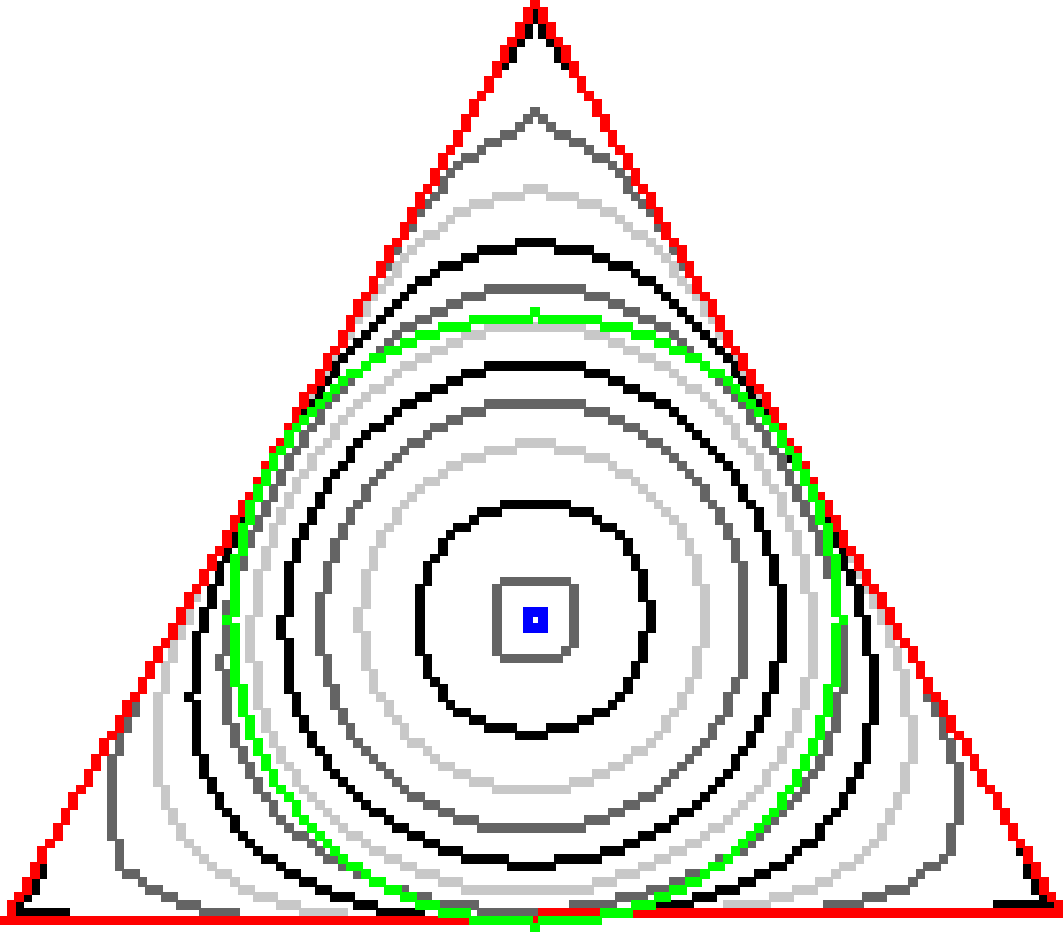
\includegraphics[scale=0.25]{figures/chapter8/graph-flow/triangle/neigh-0/alpha-0.01/summary.pdf} & 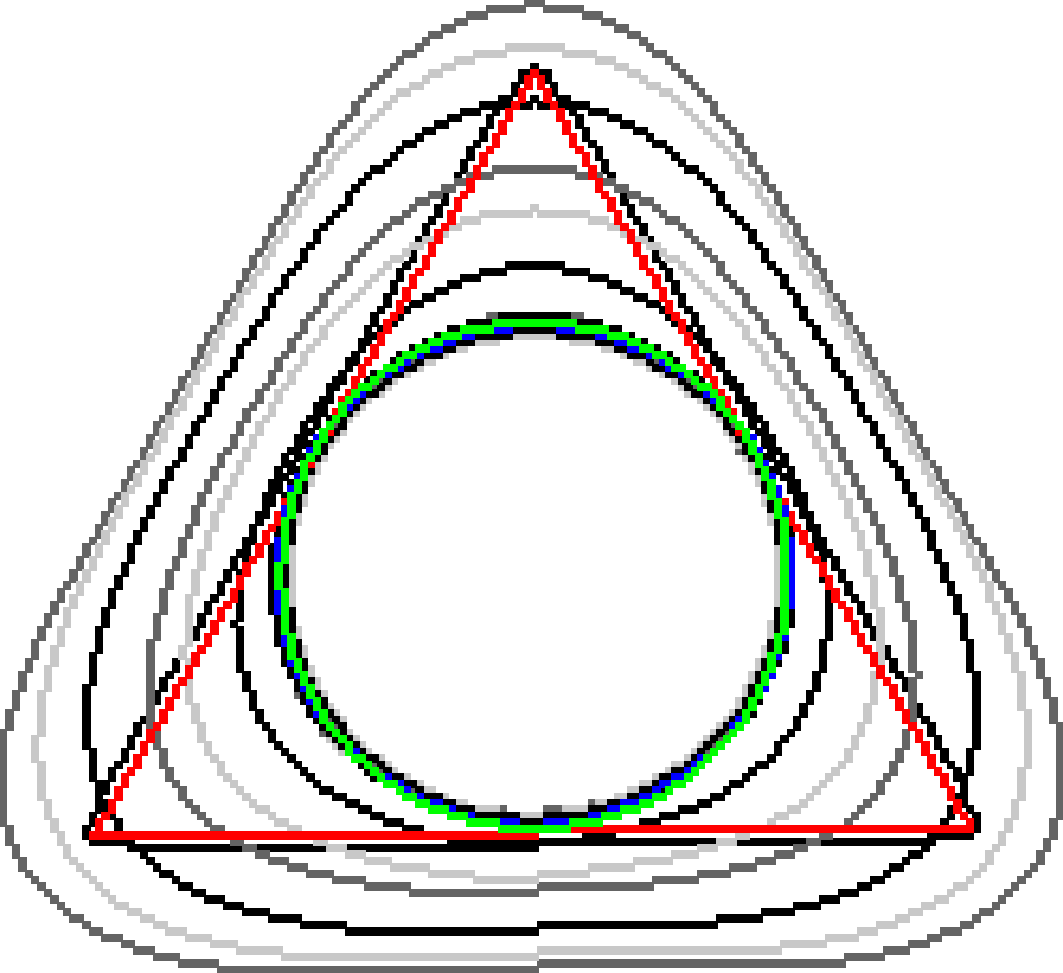
\includegraphics[scale=0.25]{figures/chapter8/graph-flow/triangle/neigh-2/alpha-0.01/summary.pdf} & 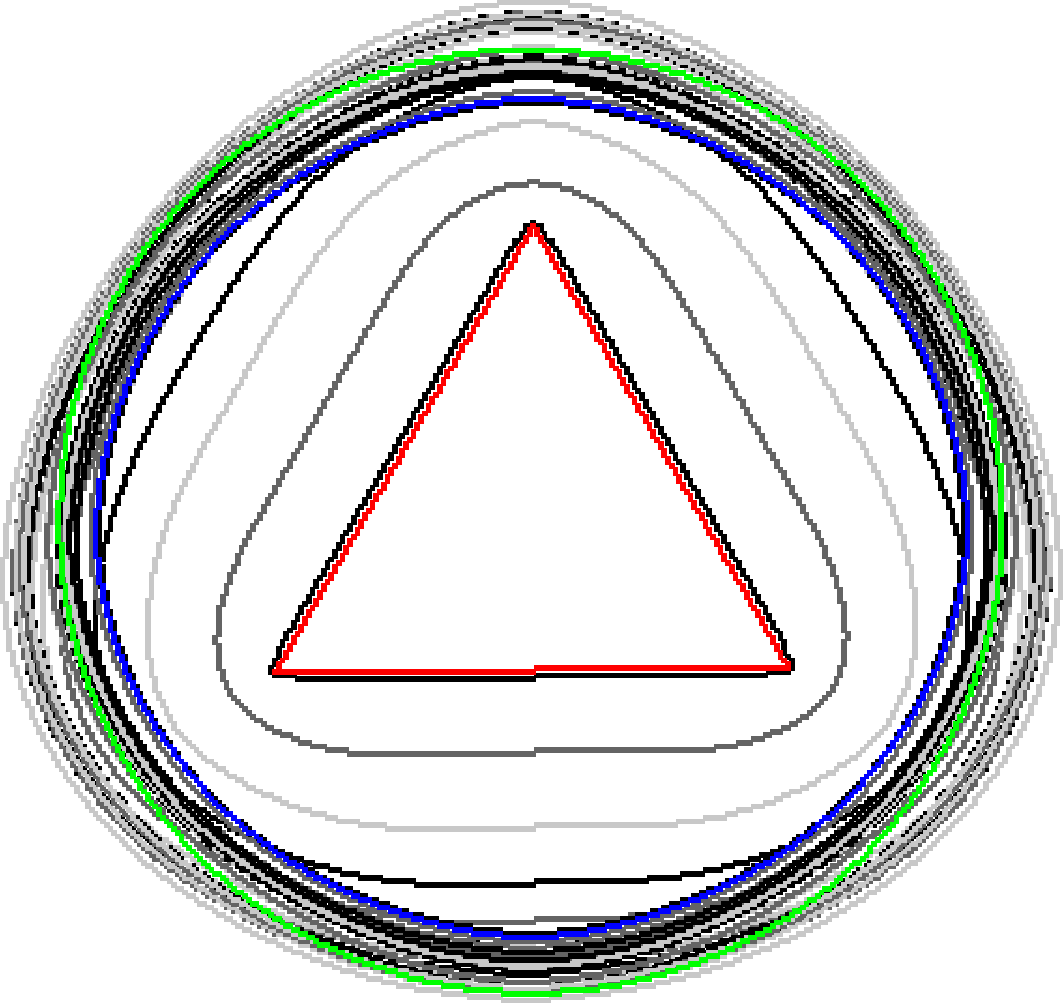
\includegraphics[scale=0.25]{figures/chapter8/graph-flow/triangle/neigh-2/alpha-0.001/summary.pdf}\\
$(n=2, a=0,\alpha=0.01)$ & $(n=2, a=2,\alpha=0.01)$ & $(n=2, a=2, \alpha=0.001)$
\end{tabular}}

\subfloat[$(n=2, a=2, \alpha=0.001)$]{
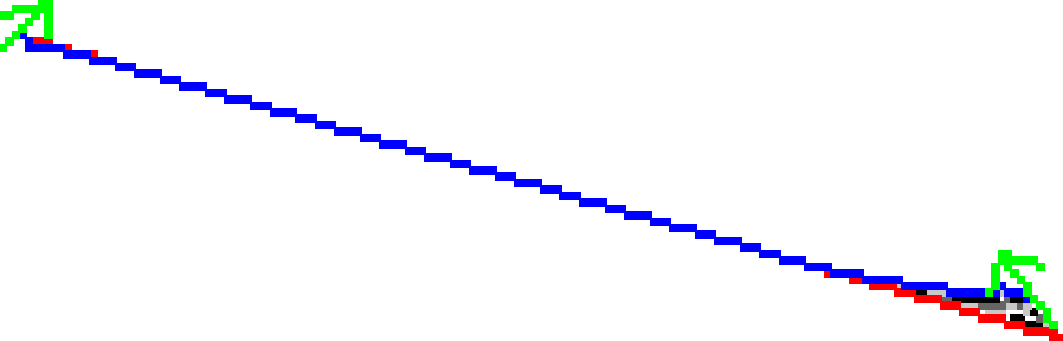
\includegraphics[scale=0.4]{figures/chapter8/constrained-elastica/curve-3/lp-0.001/summary.pdf}
}

\caption{The LSGF algorithm can shrink and grow accordingly with length penalization and it converges to shape closer to the global optimum (green curve) in the free Elastica problem. In the constrained Elastica, we believe that we can improve the results by using a larger, possibly random, neighborhood. We are using $a=2$ and shapes are displayed at every $10$ iterations.}
\label{fig:graph-flow-neigh2-results}
\end{figure}

%\section{Injecting data term}
%
%The GrabCut model (see~\cref{app:grabcut-model}) is the state-of-art graph-based technique for image segmentation tasks . The GrabCut model possesses two data term components, one related to the boundary, and another to the region. Several works tried to inject geometric information in a graph-cut framework for image segmentation. While some works were sucessfuly in injecting perimeter penalization, those that attempt to include curvature suffered from lack of precision, lack of theoretical guarantees and high running times. In this section we propose a model that advances in these two criterias.
%
%Let $I:\Omega \rightarrow [0,1]^3$ a color image. We define $I(O_m)$ as the subset of $I$ restricted to the optimization region $O_m$. Let $X_m = X(I(O_m))$ and $x$ a possible binary assignment. We recall the GrabCut minimization energy for given parameters $\Lambda=(\lambda_r, \lambda_b)$, image $I$ and labeling $x$.
%
%\begin{align*}
%	grabc_{\Lambda}(I,x) &= \lambda_r \sum_{p \in \Omega}{regional(I,x,p)} + \lambda_b \sum_{p,q \in \Omega}{boundary(I,x,p,q)}.
%\end{align*}
%
%To construct the graph $G(\mathcal{V},\mathcal{E})$, we define the edge's weight function $w$ such that curvature and data terms are contemplated. Therefore,  
%
%\[
%	\forall p,q \in O_m, \quad w(v_p,v_q) = \left\{ \begin{array}{ll}
%		\beta(u(S,p) + u(S,q)) + \lambda_b boundary(I,x,p,q), & \text{if } p,q \notin T	\\
%		\beta M + \lambda_r regional(I,x,p,q), & \text{if } p \in T \text{ xor } q \in T \\
%		0, & \text{otherwise}
%	\end{array},\right.
%\]
%
%The validation function is defined as
%
%\begin{align*}
%val_{(\Theta,\Lambda)}(S^{(k-1)},I,x^{(k-1)}) &= \hat{E}_{\Theta}(S) + grabc_{\Lambda}(I,x)
%\end{align*}
%
%Finally, the squared curvature correction algorithm is described as
%
%\begin{algorithm}
% \SetKwData{It}{k}
% \SetKwData{MIt}{maxIt}
% \SetKwData{Delta}{delta}
% \SetKwData{Tol}{tolerance}
% \SetKwInOut{Input}{input}\SetKwInOut{Output}{output}
% \SetKwComment{comment}{//}{}
% 
% \Input{A digital set $S$; the optimization band $m$; the neighborhood explorer set size $a$;  parameter vector $\Theta=(\alpha,\beta)$; data term coefficients $\Lambda=(\lambda_r,\lambda_b)$; tolerance $tolerance$.}
% \BlankLine
% $S^{(0)} \longleftarrow S$\;
% $k \longleftarrow 1$\;
% \Delta $\longleftarrow +\infty$\;
% \While{ \It $<$ \MIt \bf{and} \Delta $>$ \Tol  }{ 	
%	$candidates \longleftarrow \{\}$\;
%	\comment{Candidate selection}
% 	\ForEach{ $X \in N_a(S^{(k)})$ }
% 	{
% 		$candidates \longleftarrow candidates \cup x\big( \; \{ p \; | \; v_p \in C_s( X ) \} \; \big)$\;
% 	}
%
%	\comment{Candidate validation}
%	$S^{(k)} \longleftarrow \displaystyle \argmin_{x \in candidates}{ val_{(\Theta,\Lambda)}(S^{(k-1)},I,x^{(k-1)})}$\; 	
%	\It $\longleftarrow$ \It $+1$\;
%	\Delta $\longleftarrow | val_{(\Theta,\Lambda)}(S^{(k)},I,x^{(k)}) - val_{(\Theta,\Lambda)}(S^{(k-1)},I,x^{(k-1)}) |$\;
%	
% }
% \caption{LSGF squared curvature segmentation correction algorithm.}
% \label{alg:legc-segmentation-algorithm}  
%\end{algorithm}


\begin{figure}
\center
\begin{tabular}{cccc}
\multirow{2}{*}{Seeds} & \multirow{2}{*}{GrabCut} & $\alpha=0.5, \beta=0.0,$ & $\alpha=0.5, \beta=1.0,$\\
& & $\lambda_r=\lambda_b=2.0$ & $\lambda_r=\lambda_b=2.0$\\
 	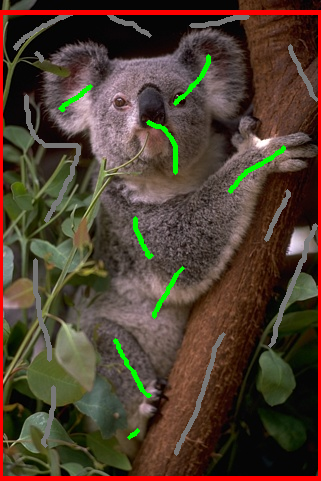
\includegraphics[scale=0.25]{figures/chapter8/segmentation/coala/k-0.0/seeds.png} & 
 	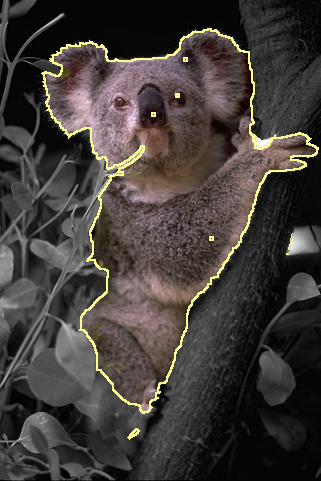
\includegraphics[scale=0.25]{figures/chapter8/segmentation/coala/k-0.0/gc-seg.png} &  	
 	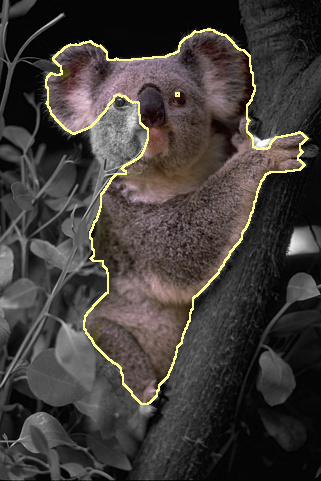
\includegraphics[scale=0.25]{figures/chapter8/segmentation/coala/k-0.0/corrected-seg.png} &  	
 	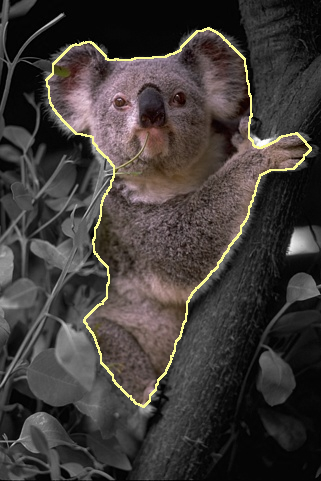
\includegraphics[scale=0.25]{figures/chapter8/segmentation/coala/k-1.0/corrected-seg.png}
\end{tabular}	
\caption{Given foreground (green) and background (gray) seeds at picture (a); GrabCut produces picture (b) which is used as input of the GraphFlow Contour Correction algorithm; in pictures (c) and (d) we display the output of Contour Correction algorithm with and without squared curvature regularization. }
\label{fig:ch8-segmentation}
\end{figure}

\begin{figure}
\center
\begin{tabular}{cc}
$\alpha=0.01, \mathbf{\beta=0}$ & $\alpha=0.01, \mathbf{\beta=1}$\\
$\lambda_r = 3, \lambda_b = 3$ & $\lambda_r = 3, \lambda_b = 3$\\
 	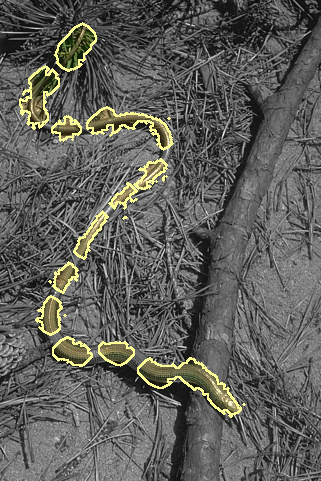
\includegraphics[scale=0.25]{figures/chapter8/completion/graphseg/alpha-0.0/beta-0.0/gamma-3.0/radius-5/corrected-seg.png} & 
 	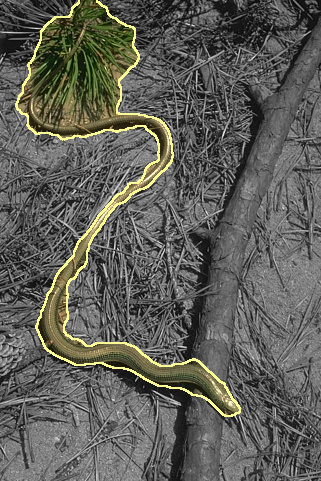
\includegraphics[scale=0.25]{figures/chapter8/completion/graphseg/alpha-0.01/beta-1.0/gamma-3.0/radius-3/corrected-seg.png}
\end{tabular}	
\caption{Completion property. The left figure illustrates an example of oversegmentation that may occur when the squared curvature term is set to zero. In the right figure, the same image is segmented as a single object when $\beta = 1$. }
\label{fig:ch8-segmentation-curvature-completion}
\end{figure}

\section{Conclusion}
A graph-cut model  We described a graph-cut model that regularizes the squared curvature, in the free, constrained Elastica and is suitable for image segmentation. The evolution produced by the GraphFlow responds to the length penalization term $\alpha$, i.e., the shape tends to grow (shrink) for lower (higher) values of $\alpha$.  Moreover, the GraphFlow~\cref{alg:graphflow-algorithm} is faster and simpler to implement than the previous models presented in this thesis.